\documentclass[10pt]{exam}
\usepackage[phy]{template-for-exam}
\usepackage{hyperref,cclicenses,graphicx}

\title{Geometric Optics (Lenses) PhET Simulation}
\author{Rohrbach}
\date{\today}

\begin{document}
\maketitle

\hrule
\vspace{0.2em}
\noindent
{\footnotesize Worksheet adapted from \emph{Optics Online Worksheet} by Scott McCurdy }

{\footnotesize License:} \cc\hspace{-1em}\ccby  {\footnotesize CC BY: Attribution.}

{\footnotesize Retrieved 2025-06-17 from \texttt{\href{https://phet.colorado.edu/en/activities/3231}{https://phet.colorado.edu/en/activities/3231}} }
\vspace{0.2em}
\hrule

\vspace{2em}

\noindent
Go to Schoology to find the link to the Geometric Optics PhET Smiulation.  Alternatively, you can go to \href{http://phet.colorado.edu/en/simulation/geometric-optics}{\texttt{http://phet.colorado.edu/en/simulation/geometric-optics}}.

\begin{itemize}
    \item Click the ``Play'' icon for the application.
    \item Select the \textbf{Lens} option from the menu.
    \item In the bottom right corner, make sure that \emph{``focal points''}, \emph{``virtual image''}, and \emph{``labels''} are checked.
    
    \hfill  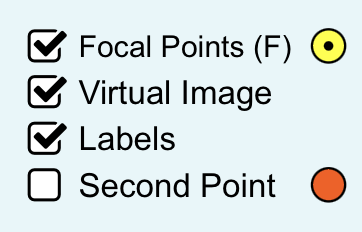
\includegraphics[height=2cm]{checkboxes.png}

\end{itemize}

\begin{questions}
    \question 
      Move the pencil on the left and observe what happens to the image. 

    \begin{parts}
      \part 
        What happens to the image as the object moves closer to the lens, but before reaching the focal point (the yellow dot)? \vs
      \part 
        What happens to the image when the object is moved in front of the focal point? \vs
      
    \end{parts}
  
    \question 
      Adjust the curvature radius and observe what happens. (Lower radius of curvature leads to a thicker lens.)

      \begin{parts}
        \part
          As the lens gets thicker, what happens to the focal point? \vs
        \part 
          What happens to the image? \vs
      \end{parts}

    \pagebreak
    
    \question 
      Select \emph{``second point''} at the bottom-right of the options bar. You should see an orange dot on the pencil and a new set of orange rays going through the lens.
     
    \begin{parts}
        \part
          Slide the dot up and down. What happens to the rays? \vs
        \part
          Place the orange dot at the center of the pencil. Where do the rays intersect? \vs
        \part
          Place the dot on the eraser. Where do the rays intersect? \vs
    \end{parts}
    
    \question 
      Deselect \emph{``second point''} and change the lens type to the \emph{diverging lens} near the top-middle of the screen.

      {\hfill 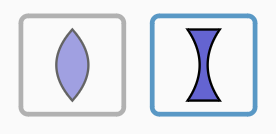
\includegraphics{lenstypes.png} \hfill}

    \begin{parts}
        \part
          What happens to the image as the object moves closer to the lens? \vs
        \part
          Can a diverging lens make a real image? Why or why not? \vs
    \end{parts}
\end{questions}


\end{document} 